% Some commands used in this file
%\newcommand{\package}{\emph}

\chapter{Autonomous Guided Vehicles \& ITU-AGVs}
\label{chap:agvs}

\begin{figure}[h]
	\centering
	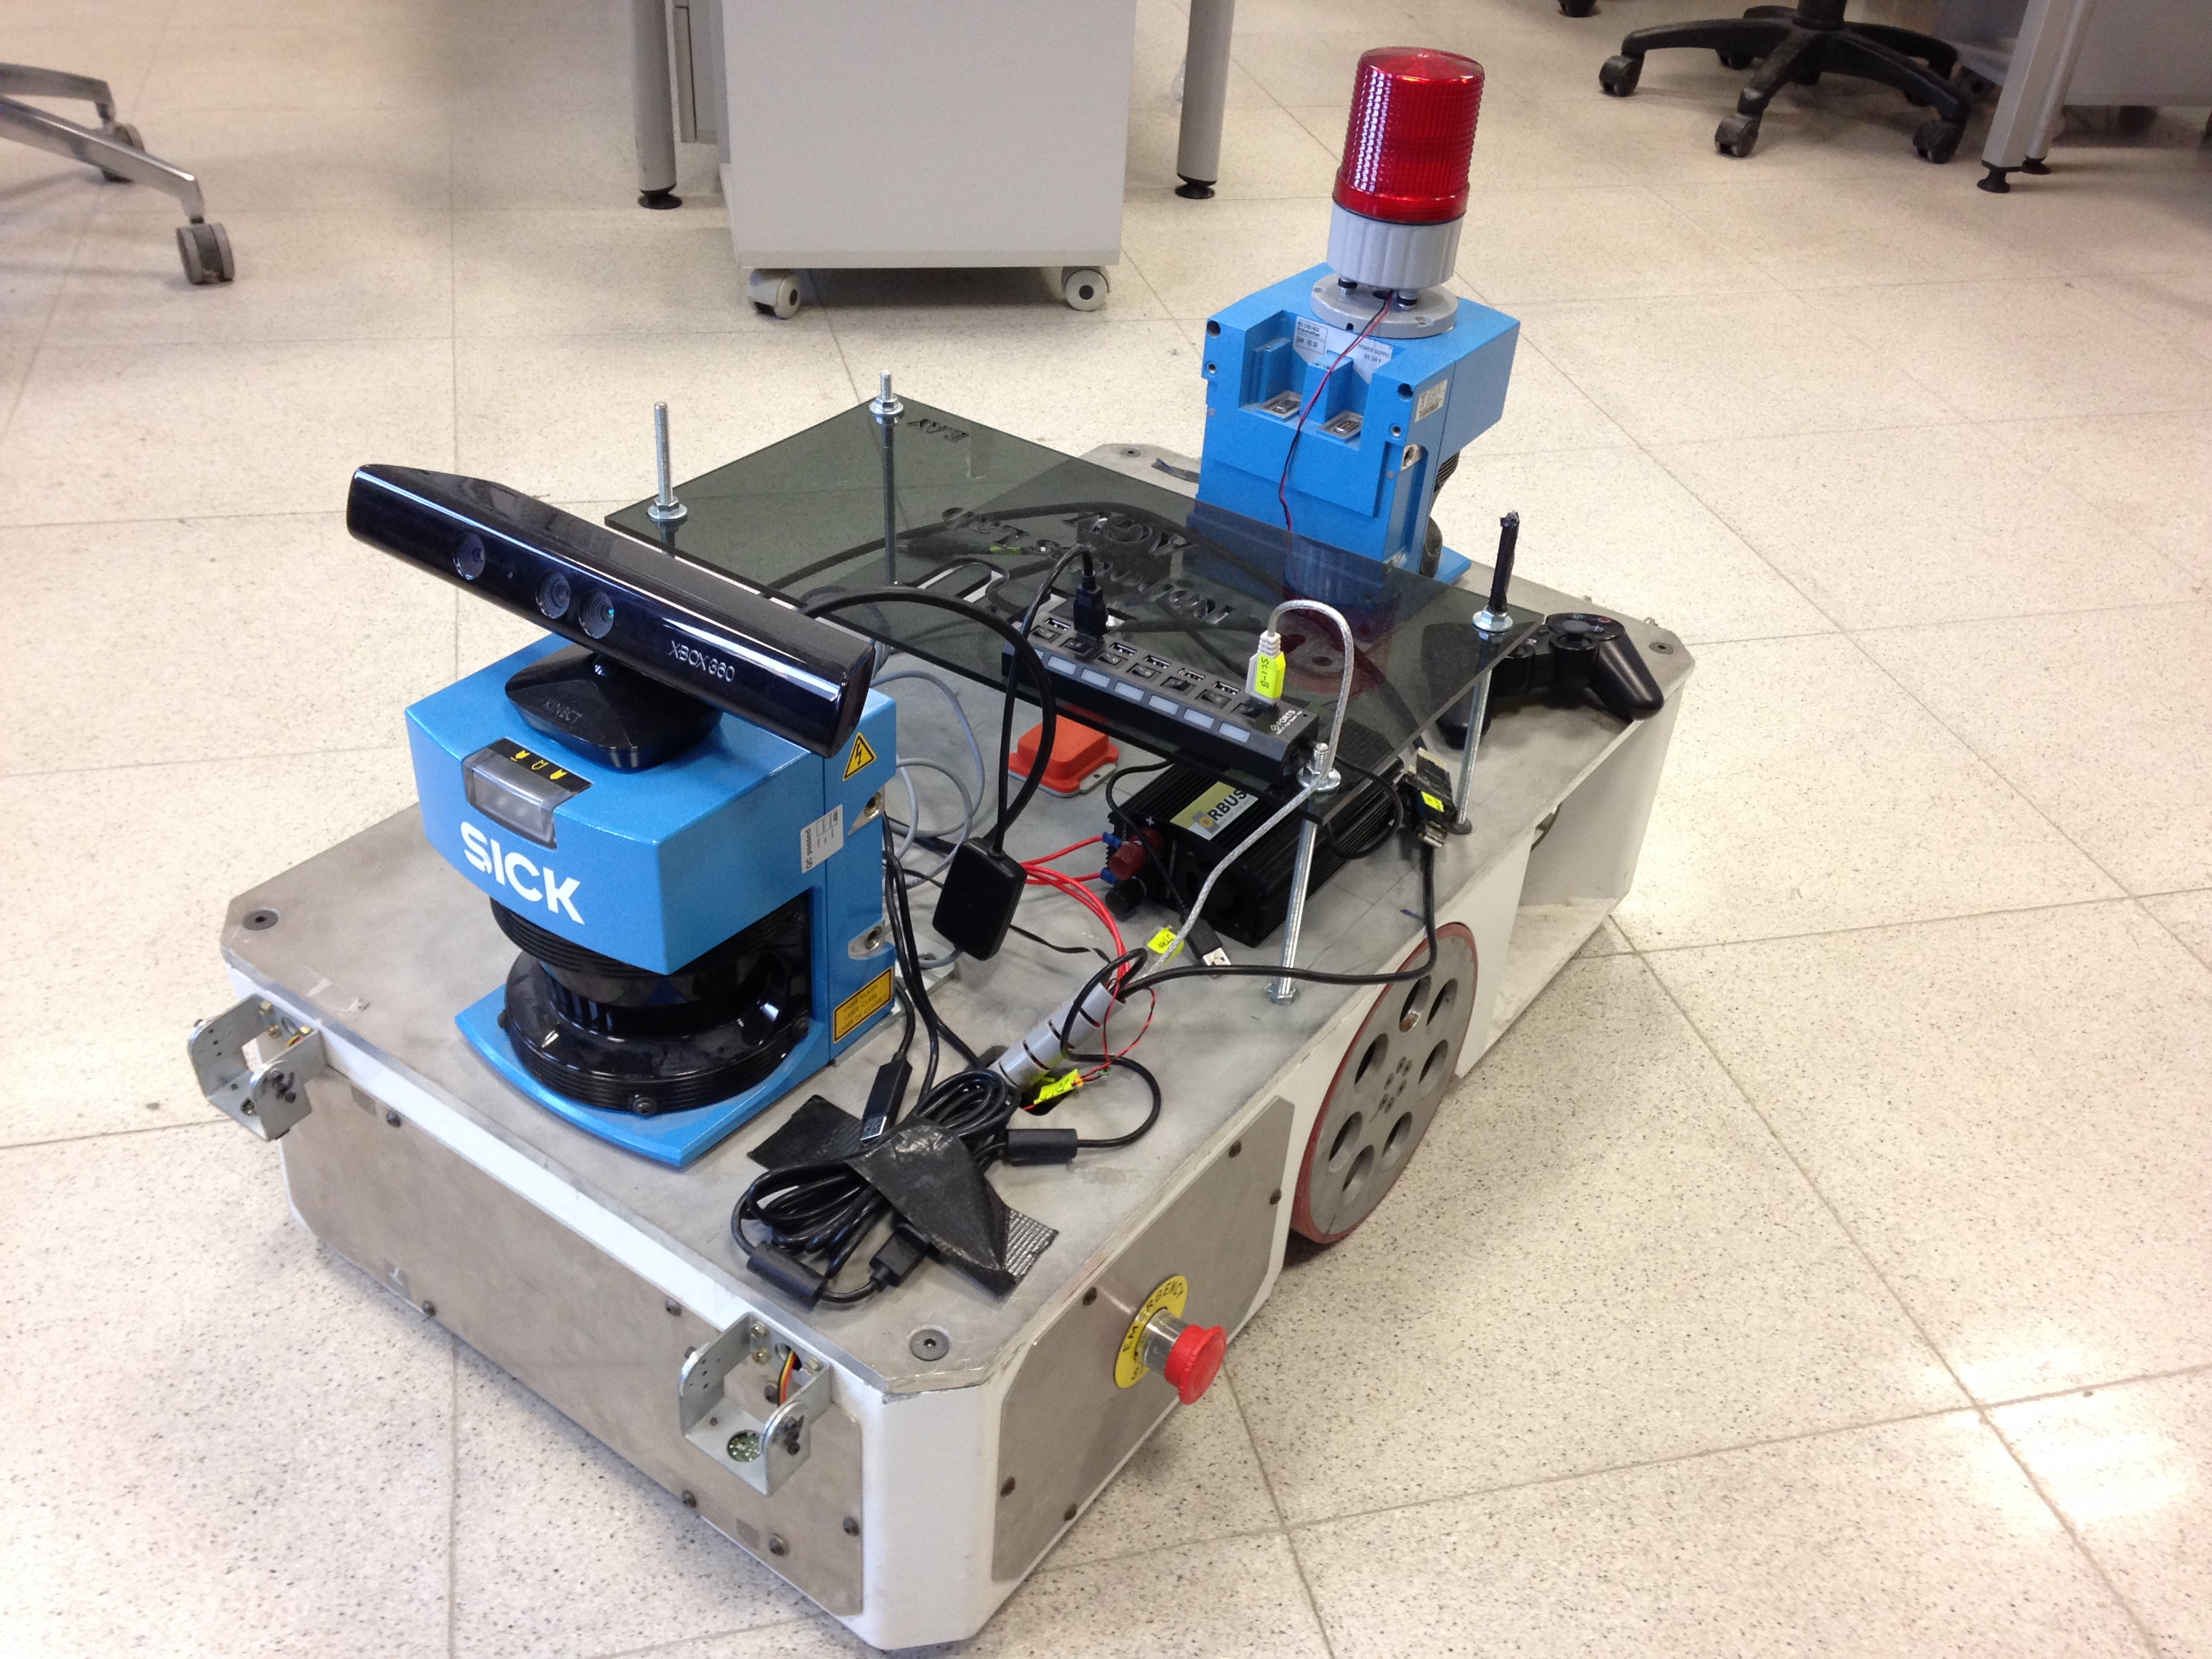
\includegraphics[scale=0.11]{images/agv1}
	\caption{One of the ITU-AGV robots}
	\label{fig:agv1}
\end{figure}

Autonomous Guided Vehicles (AGVs) or Automated Guided Vehicles are mobile robots that use lines or wires installed on the floor, cameras or laser sensors in order to navigate. They are industrial robots and their usual task is to carry objects or products in indoor or outdoor environments. Their market might be considered as the biggest one in mobile robotics \cite{alonzoKelly}. The present-day AGVs are mostly use laser sensors instead of floor wires or lines. 
\par
There are two identical AGVs that have built at Istanbul Technical University Robotics Laboratory named ITU-AGVs. Although they are designed as AGVs, they do not necessarily have to be used for warehouse automation or object carrying, but also they can be used as multi-purpose wheeled mobile robots. 

\section{Spesifications of ITU-AGVs}
\label{sec:specs of agvs}
ITU-AGV robots are differential-driven, bidirectional mobile robots with two driving wheels and two caster wheels (Figure ~\ref{fig:agv1}). They have two 250 Watt Maxon EC54 brushless DC motors with a ratio of 1:100 reduction gear-boxes. The motors are driven by using Maxon EPOS 70/10 drivers. The robots are powered with two serially connected batteries with 12 V output voltage and 26 Ah charge, each. To supply motors and all other hardware, there are 5 V, 12 V and 24 V voltage regulators in order to acquire necessary voltage levels. 
\par
ITU-AGVs have 49 cm width, 82 cm length and 22 cm height. The driving wheels have 10 cm radius. They weight approximately 70 kg without the additional sensors and their payload is approximately 100 kg for each. 
\par
It is possible to install various sensors on the robot. To make it a multi-purpose robot that can be used in different future projects, two laser range finder sensors, a Microsoft Kinect sensor, an inertial measurement unit (IMU) and four analog distance sensors are mounted on ITU-AGVs. The microcontrollers provided for ITU-AGVs were Texas Instruments TMS320F28335 with Spectrum Digital eZdsp F28335 board. 
The power chart of ITU-AGVs can be seen in Figure ~\ref{fig:agvPower}.

\begin{figure}
	\centering
	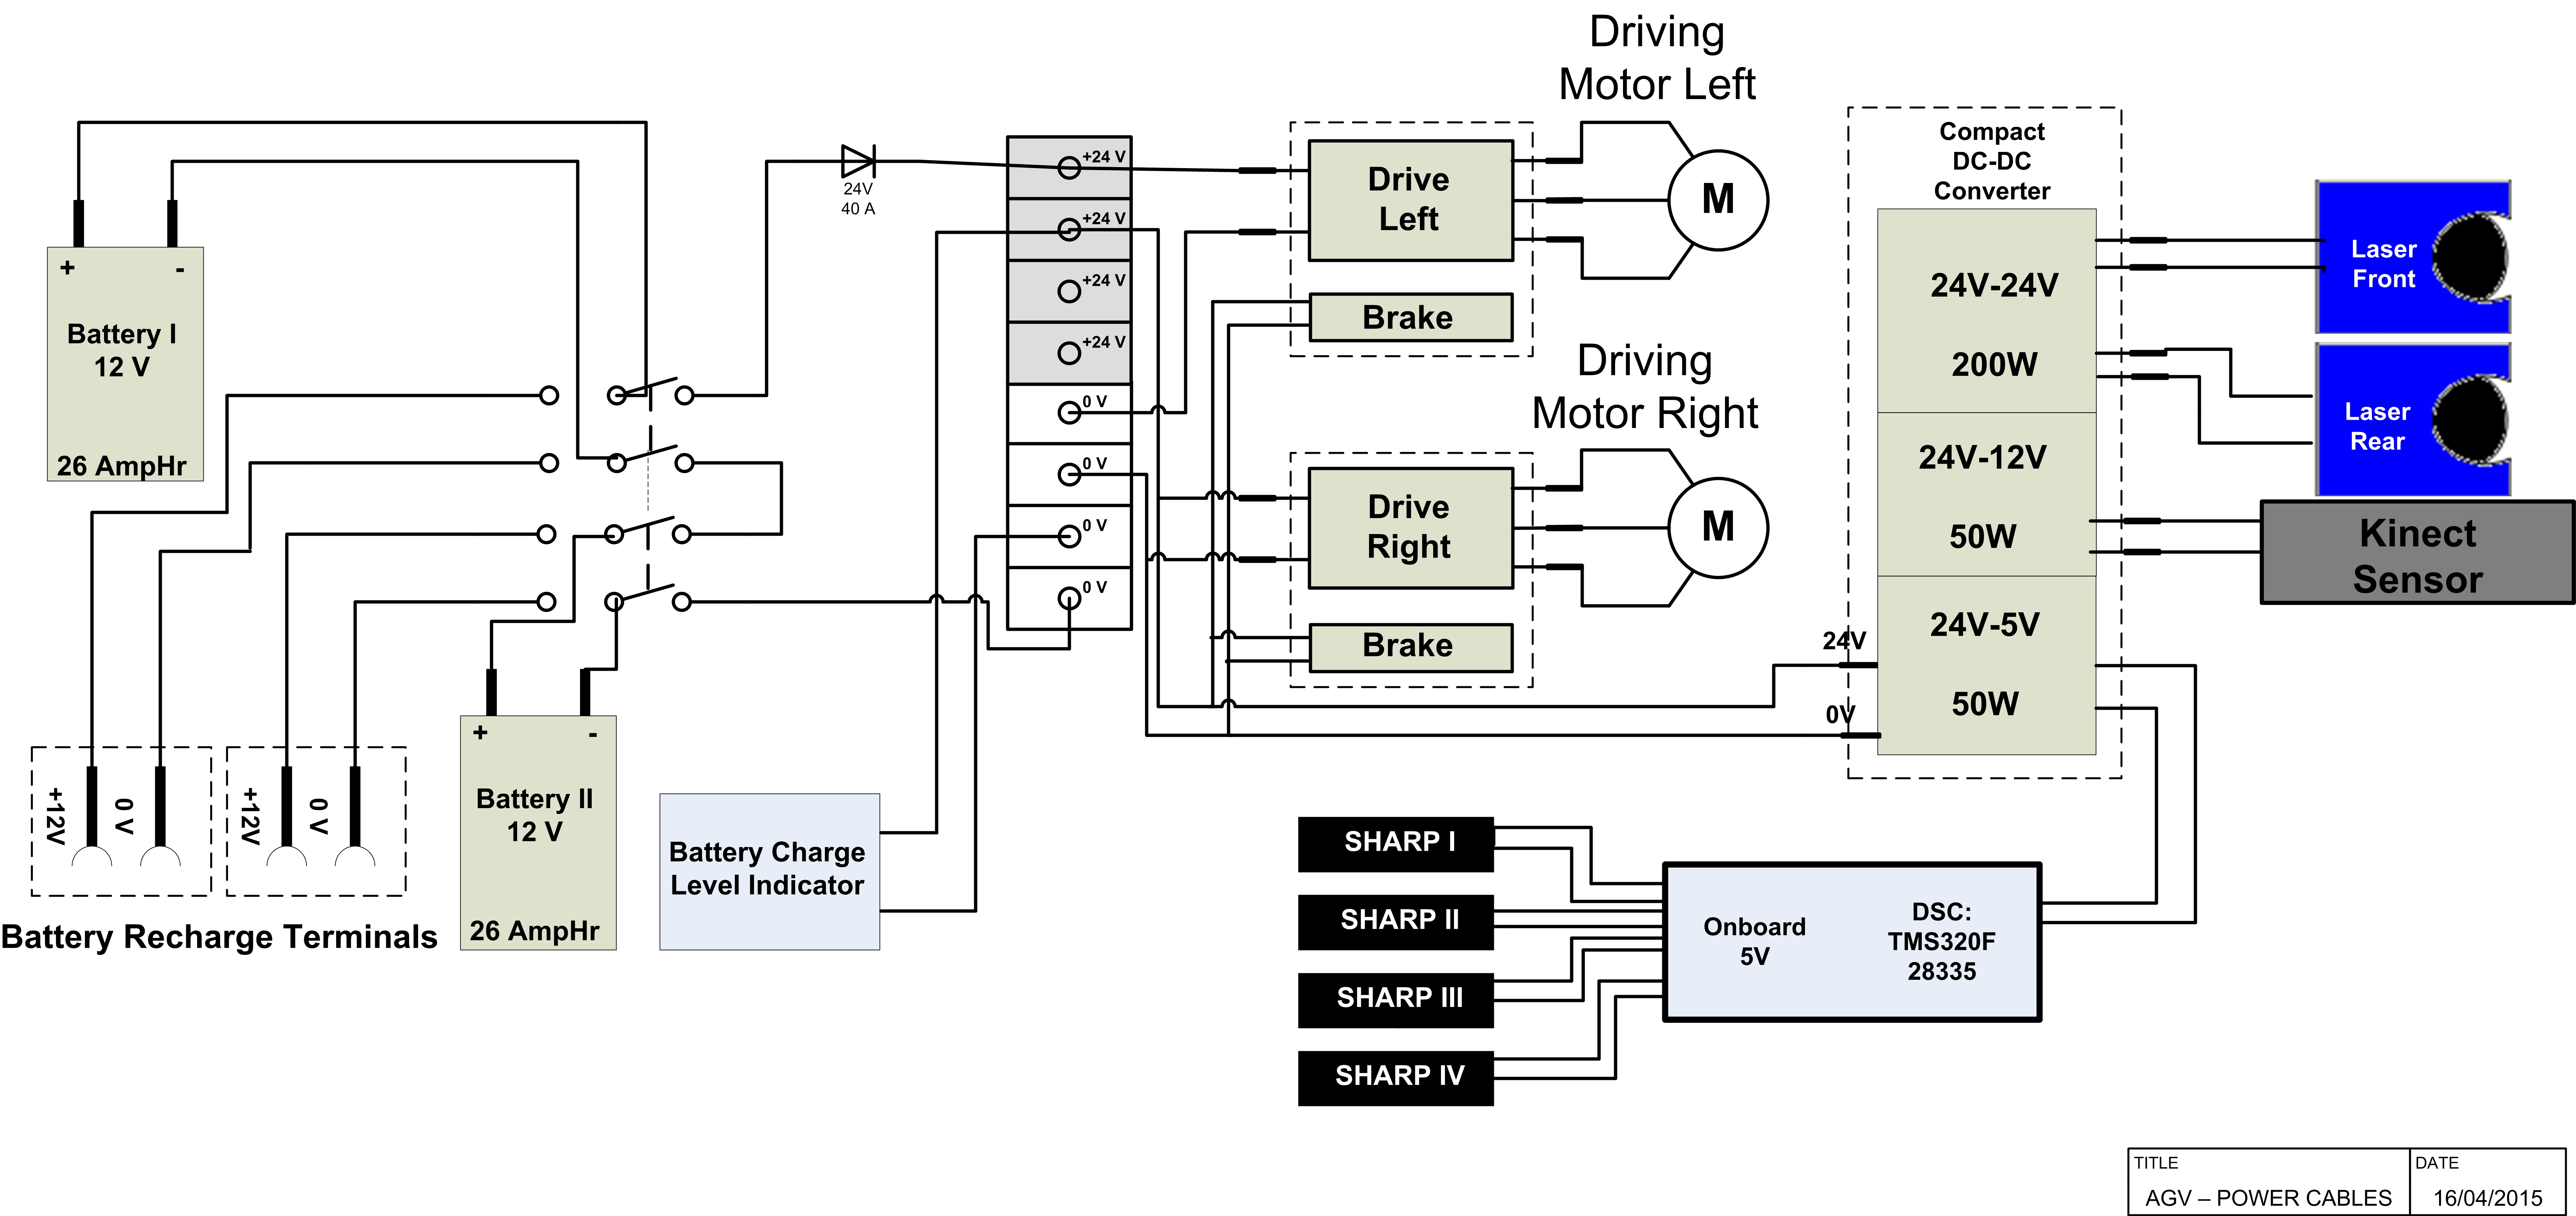
\includegraphics[scale=0.42]{images/img2-agvPower}
	\caption{Power chart of ITU-AGVs}
	\label{fig:agvPower}
\end{figure}

\section{Sensors and Low Level Processing Layer (LLPL)}
\label{sec:sensors and llpl}

\subsection{Light Detection and Ranging (LIDAR) Sensors}
\label{subsec:lidar}
There are two light detection and ranging (LIDAR) sensors mounted on ITU-AGVs. These are SICK Laser Measurement System LMS200 (Figure ~\ref{fig:kinect-sick}) and they are indoor sensors with 180 degrees scanning field and 10 meters range. Their working principle is based on time of flight measurement of reflected infrared light beam emitted by the sensor. In order to have a radial range, a rotating mirror deflects the emitted infrared light to the environment. The sensor outputs the distance values in the range for 180 degrees at 9600 baud rate ~\cite{sickDatasheet}.

\subsection{Inertial Measurement Unit (IMU)}
\label{subsec:imu}
Using an internal measurement unit is useful for position and orientation estimation. Hence, a 3 DOF Xsens MTi Attitude and Heading Reference System (AHRS) is mounted on ITU-AGVs (Figure ~\ref{fig:xsens}). Xsens MTi is an IMU that has magnetometers, accelerometers and gyroscopes and it outputs orientation, acceleration, rate of turn and earth magnetic data in three dimensions ~\cite{xsensDatasheet}. It has small dimensions ($58\times58\times22$ mm) and low weight (50 g). The sensor is mounted along the center of the robot. 

\subsection{Infrared Distance Sensors}
\label{subsec:infrared sensors}
Four infrared distance sensors are mounted on front and rear of ITU-AGVs in order to understand if there is a hole or a stair while the robots are moving in the environment. The infrared distance sensors are analog Sharp sensors with 30 cm ranges. 

\subsection{Microsoft Kinect Sensor}
\label{subsec:kinect}
Microsoft Kinect sensor has an RGB camera with $1280\times960$ resolution, an infrared emitter and infrared depth sensor to get the depth information by measuring the distance of objects from the reflected infrared beams that have emitted by the sensor, a microphone array, an accelerometer and a tilt motor ~\cite{kinectSpecs}. It is mounted on the front of ITU-AGVs (Figure ~\ref{fig:kinect-sick}) and its RGBD output can be used for many applications. 

\begin{figure}[h]
	\centering
	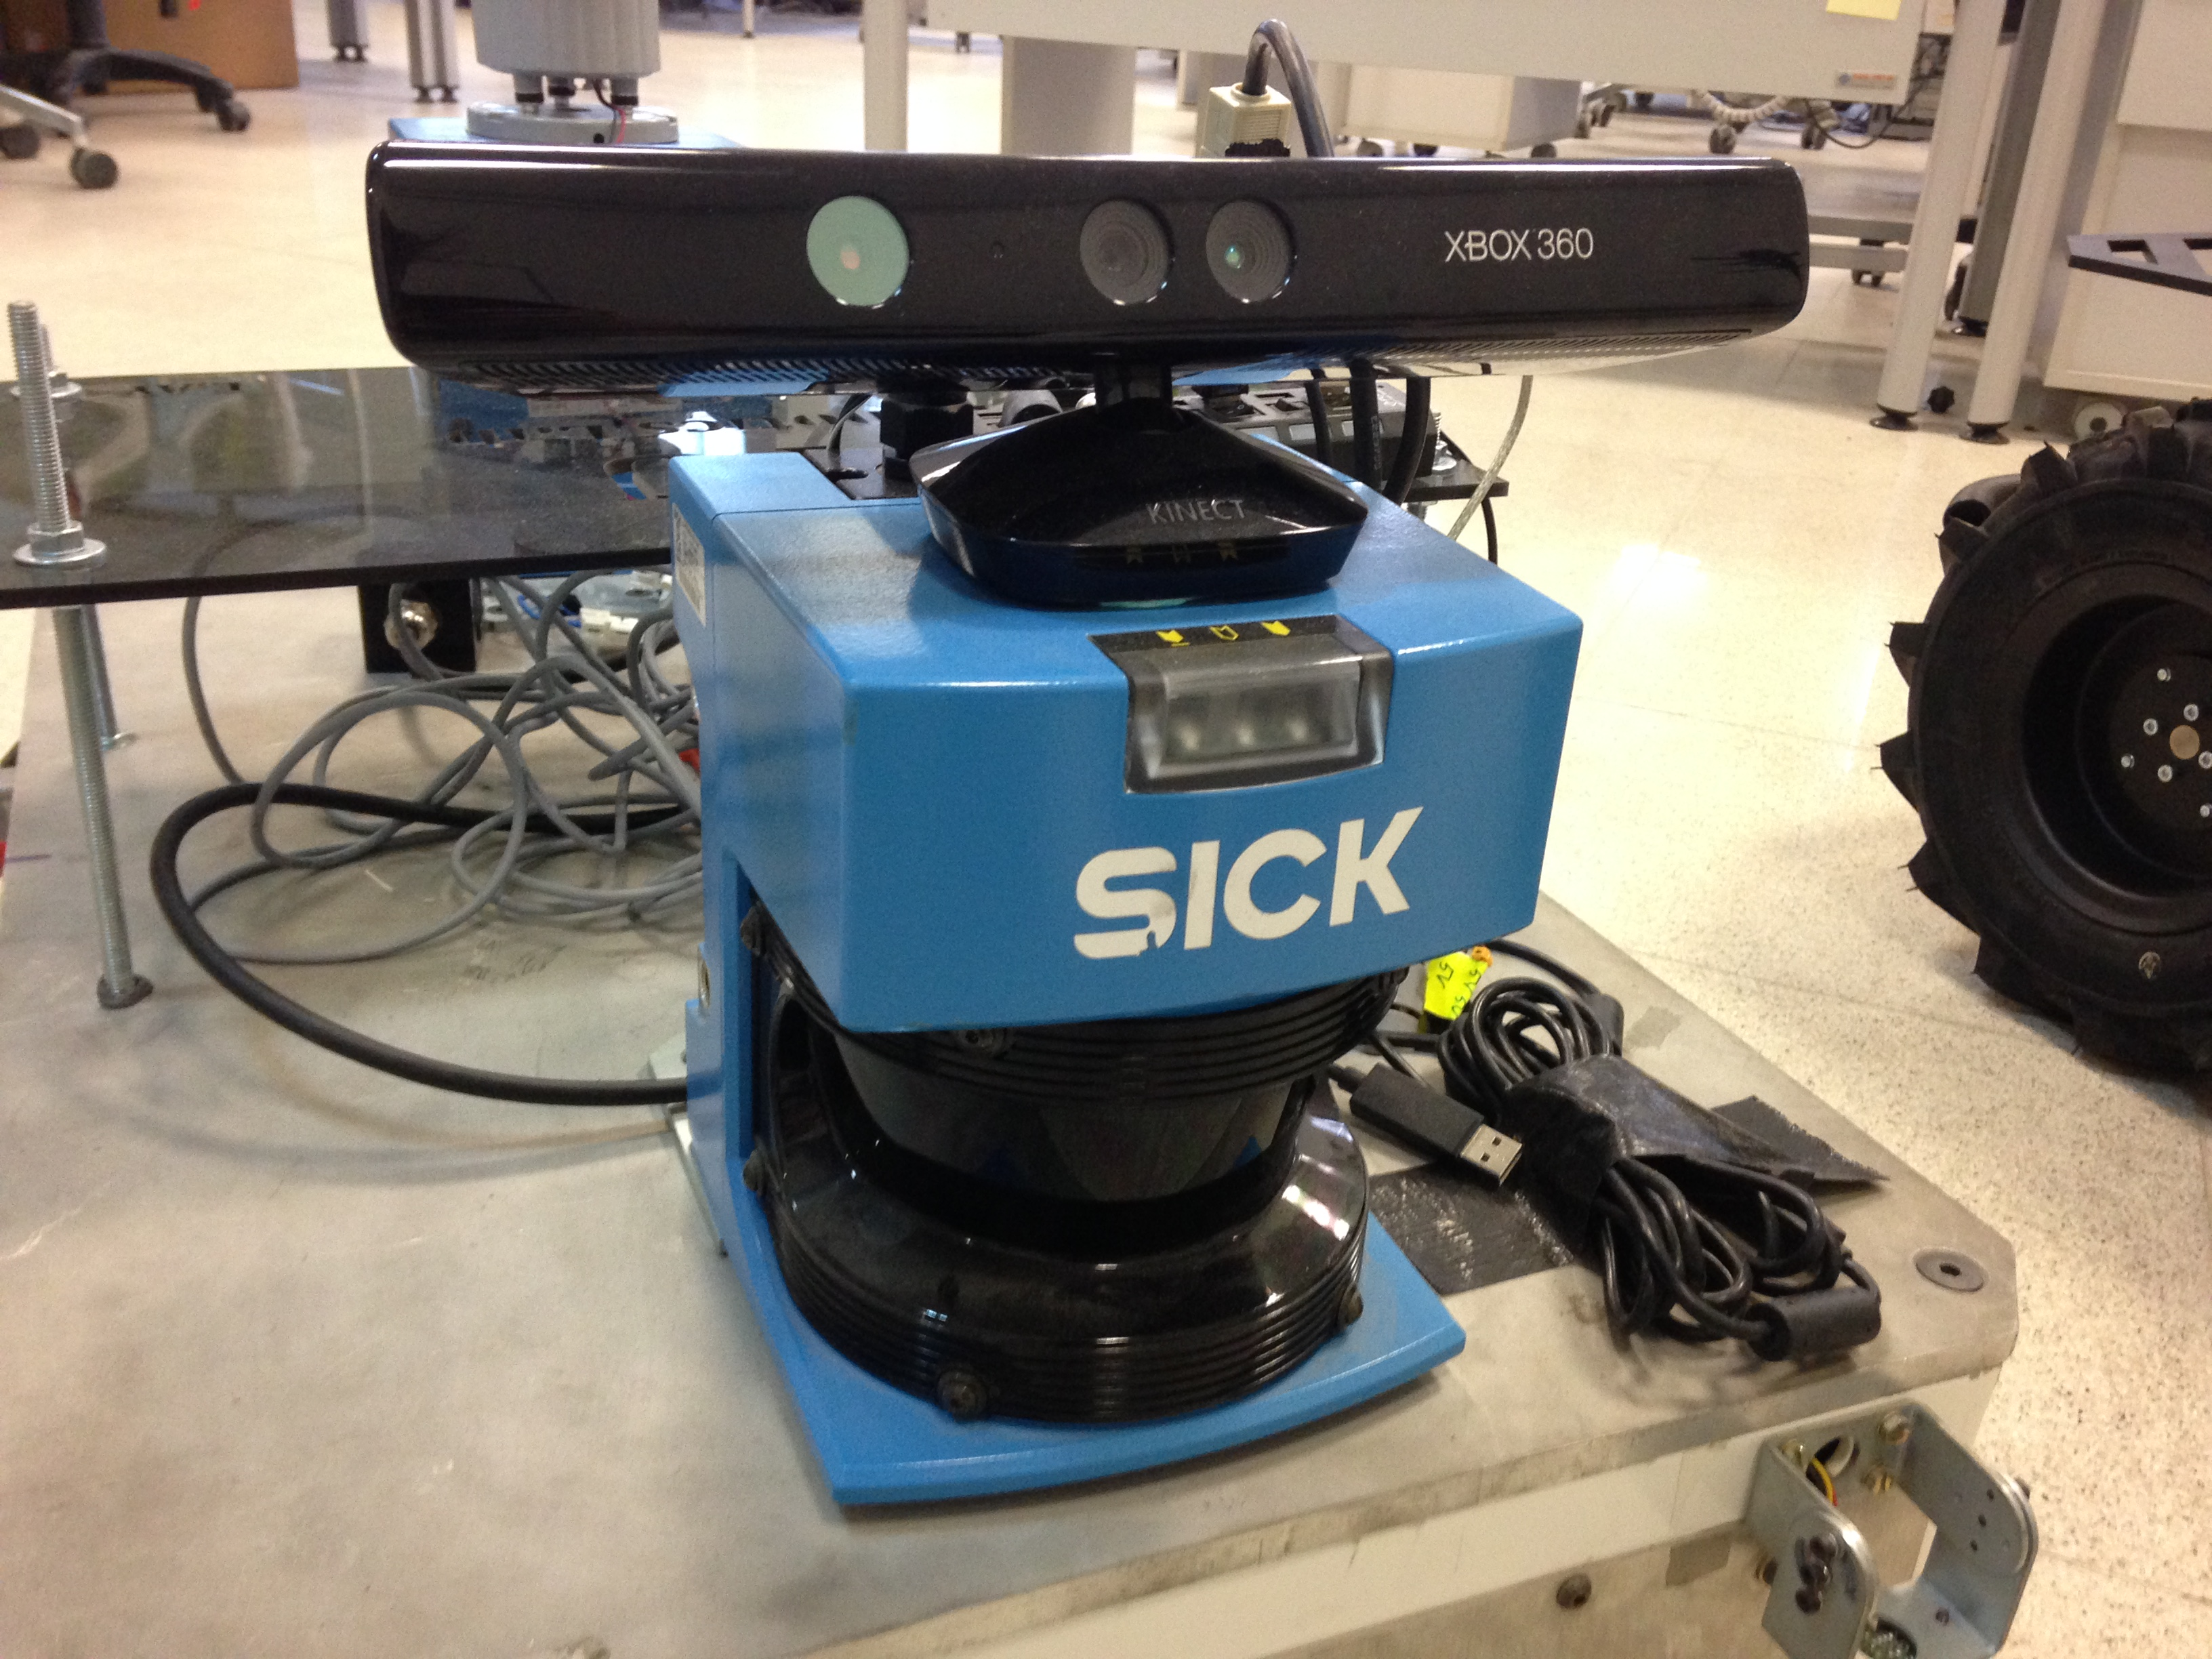
\includegraphics[scale=0.1]{images/kinect-sick}
	\caption{Microsoft Kinect and Sick LMS200 sensors on ITU-AGVs}
	\label{fig:kinect-sick}
\end{figure}

\subsection{Motor Encoders}
\label{subsec:encoder}
Motor encoders are also vital for estimation of position and orientation. The motors have three channels, 500 counts per turn HEDL 9140 encoders.

\begin{figure}
	\centering
	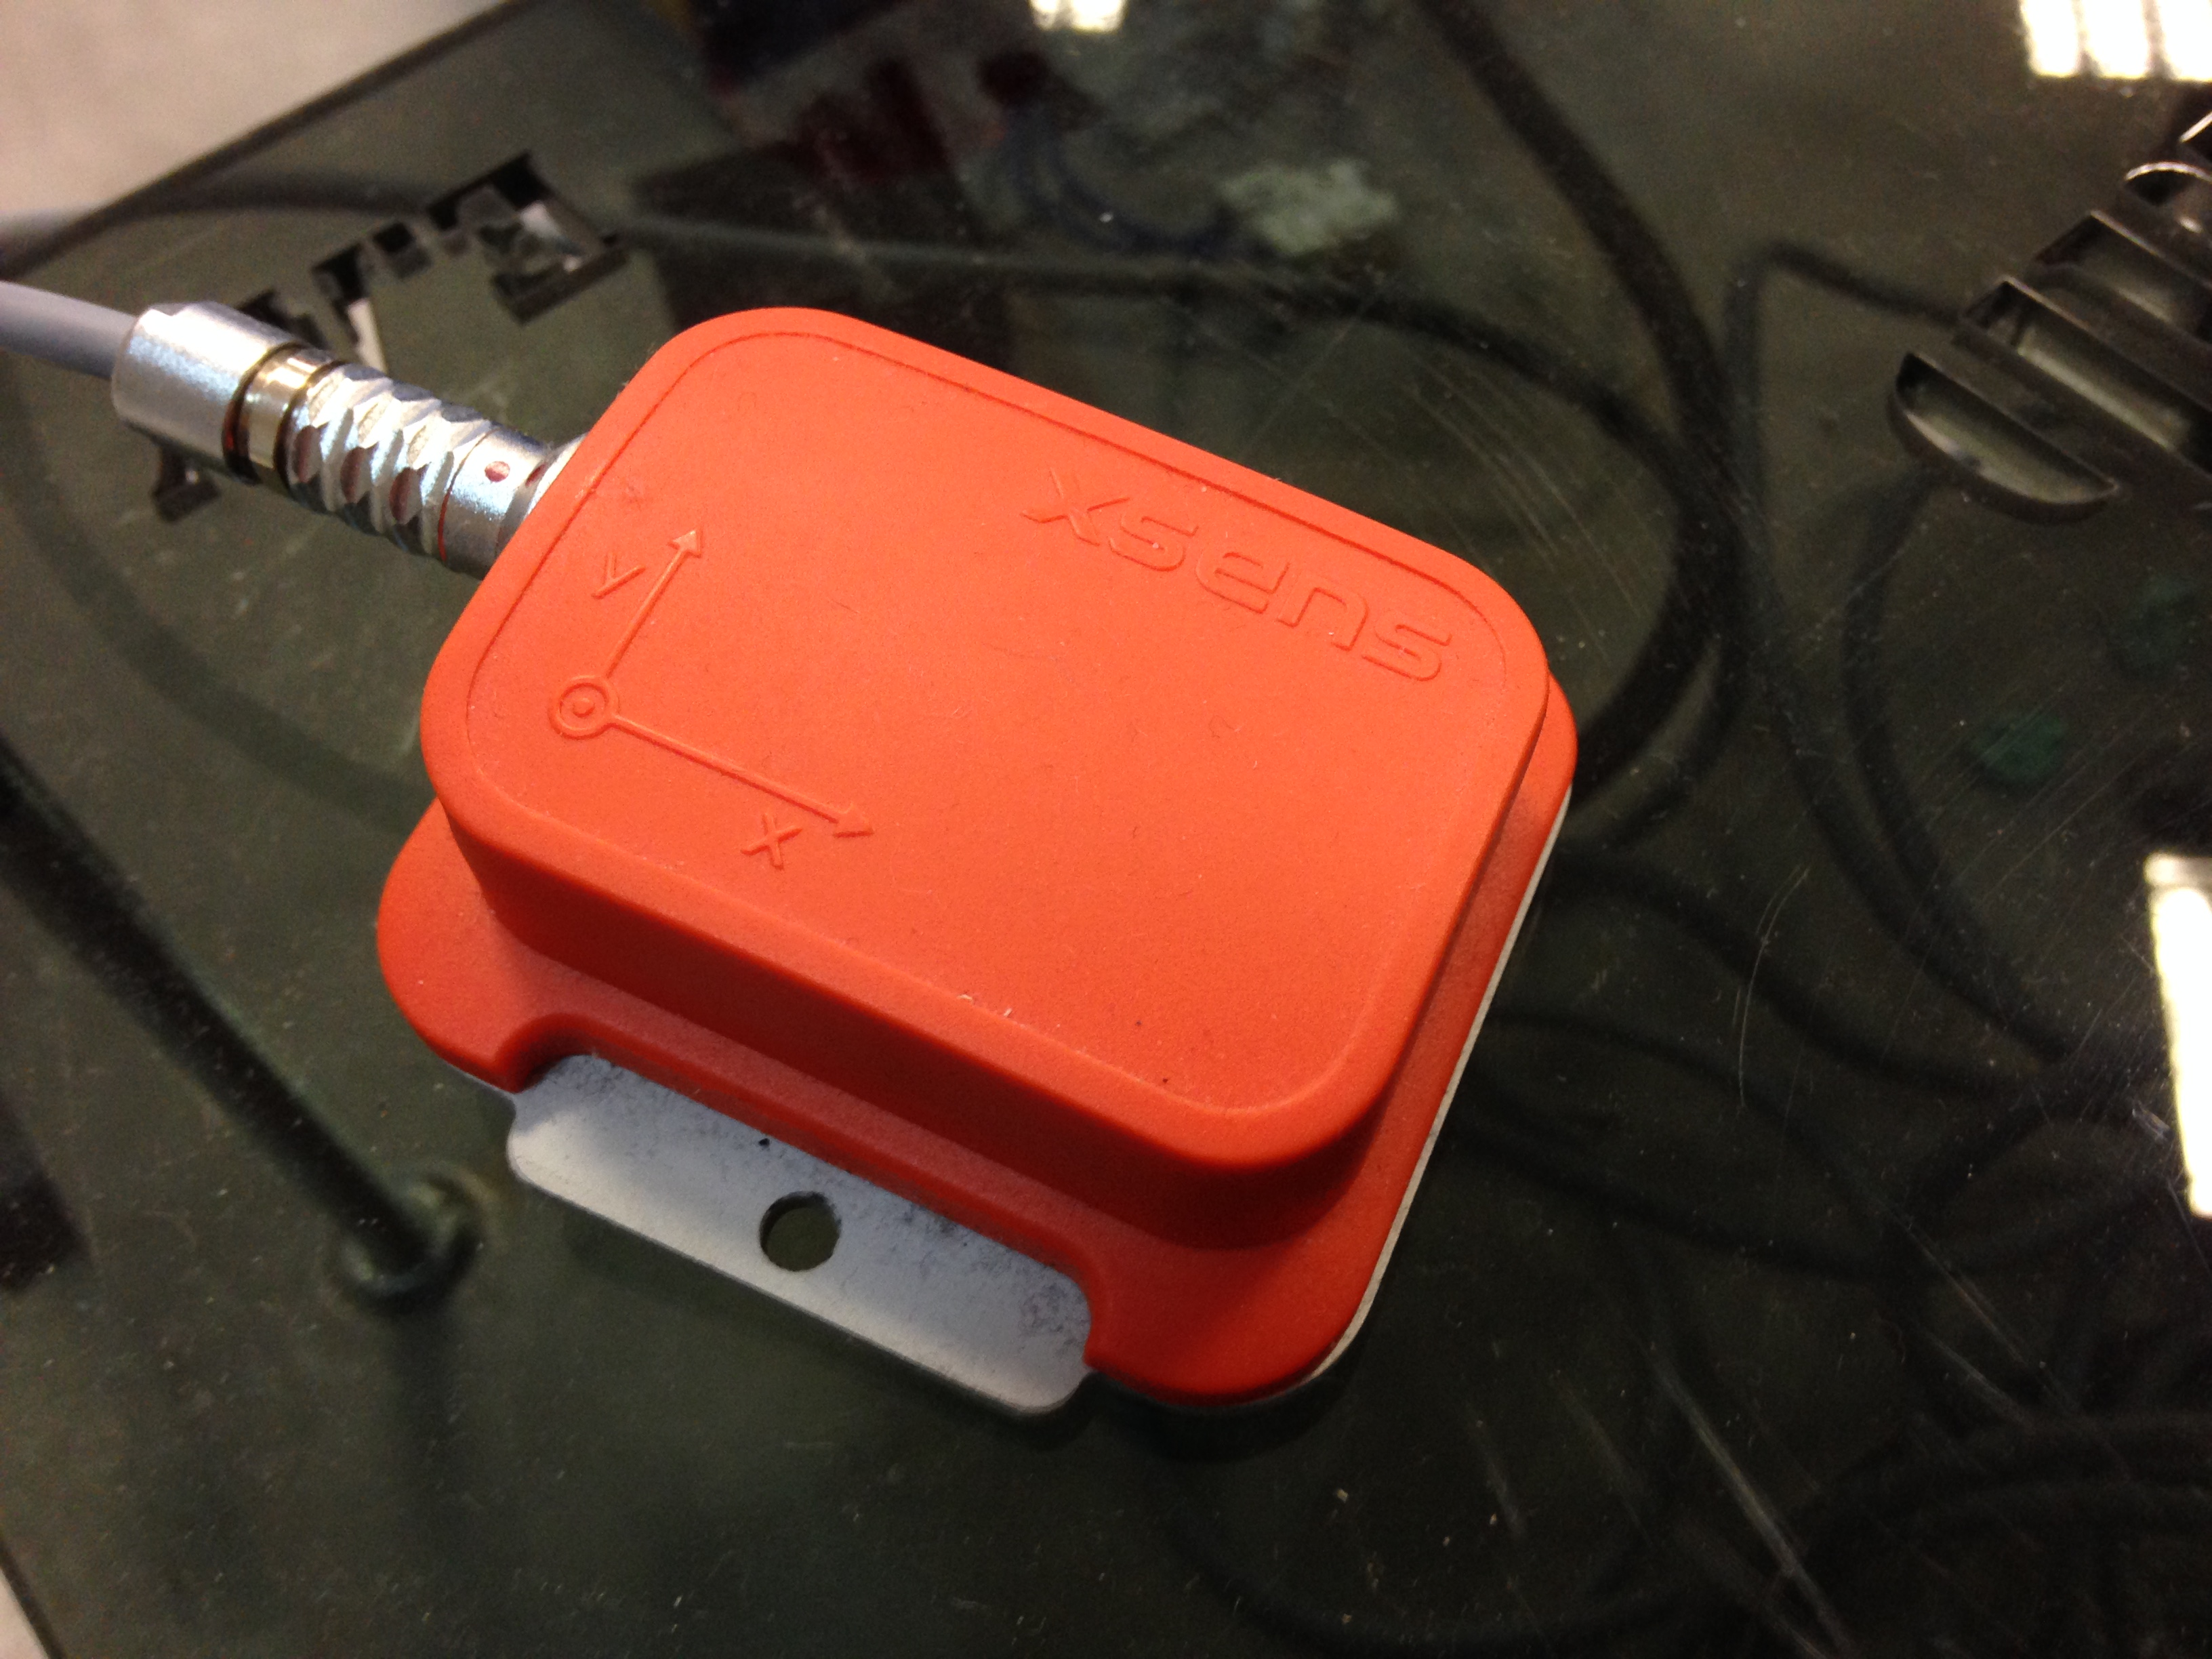
\includegraphics[scale=0.1]{images/xsens}
	\caption{Xsens MTi sensor on ITU-AGVs}
	\label{fig:xsens}
\end{figure}


\subsection{Low Level Processing Layer (LLPL)}
\label{subsec:llpl}
As in many robotic systems, there are two processing layers in ITU-AGVs. Low Level Processing Layer (LLPL) is responsible of getting commands from High Level Processing Layer (HLPL), communicating with motor drivers and sending necessary signals to drive the motors, requesting the encoder values and send them to HLPL. In addition to these flow, the analog distance sensors are also connected to LLPL. The microcontrollers used at LLPL on ITU-AGVs are Texas Instruments TMS320F28335 with Spectrum Digital eZdsp F28335 board. 
\par
The eZdsp F28335 is a stand-alone board with TMS320F28335 Digital Signal Controller. It works at 150 Mhz operating speed and it has 32-bit floating point unit, 68 KB RAM, 512 KB Flash memory, 256 KB off-chip SRAM memory, 12-bit Analog to Digital Converter (ADC), 30 MHz input clock, RS232 and CAN connectors, USB JTAG controller and multiple General Purpose Input Output (GPIO) pins~\cite{ezdspDatasheet}.


\section{Kinematics}
\label{sec:kinematics}
\begin{figure}
	\centering
	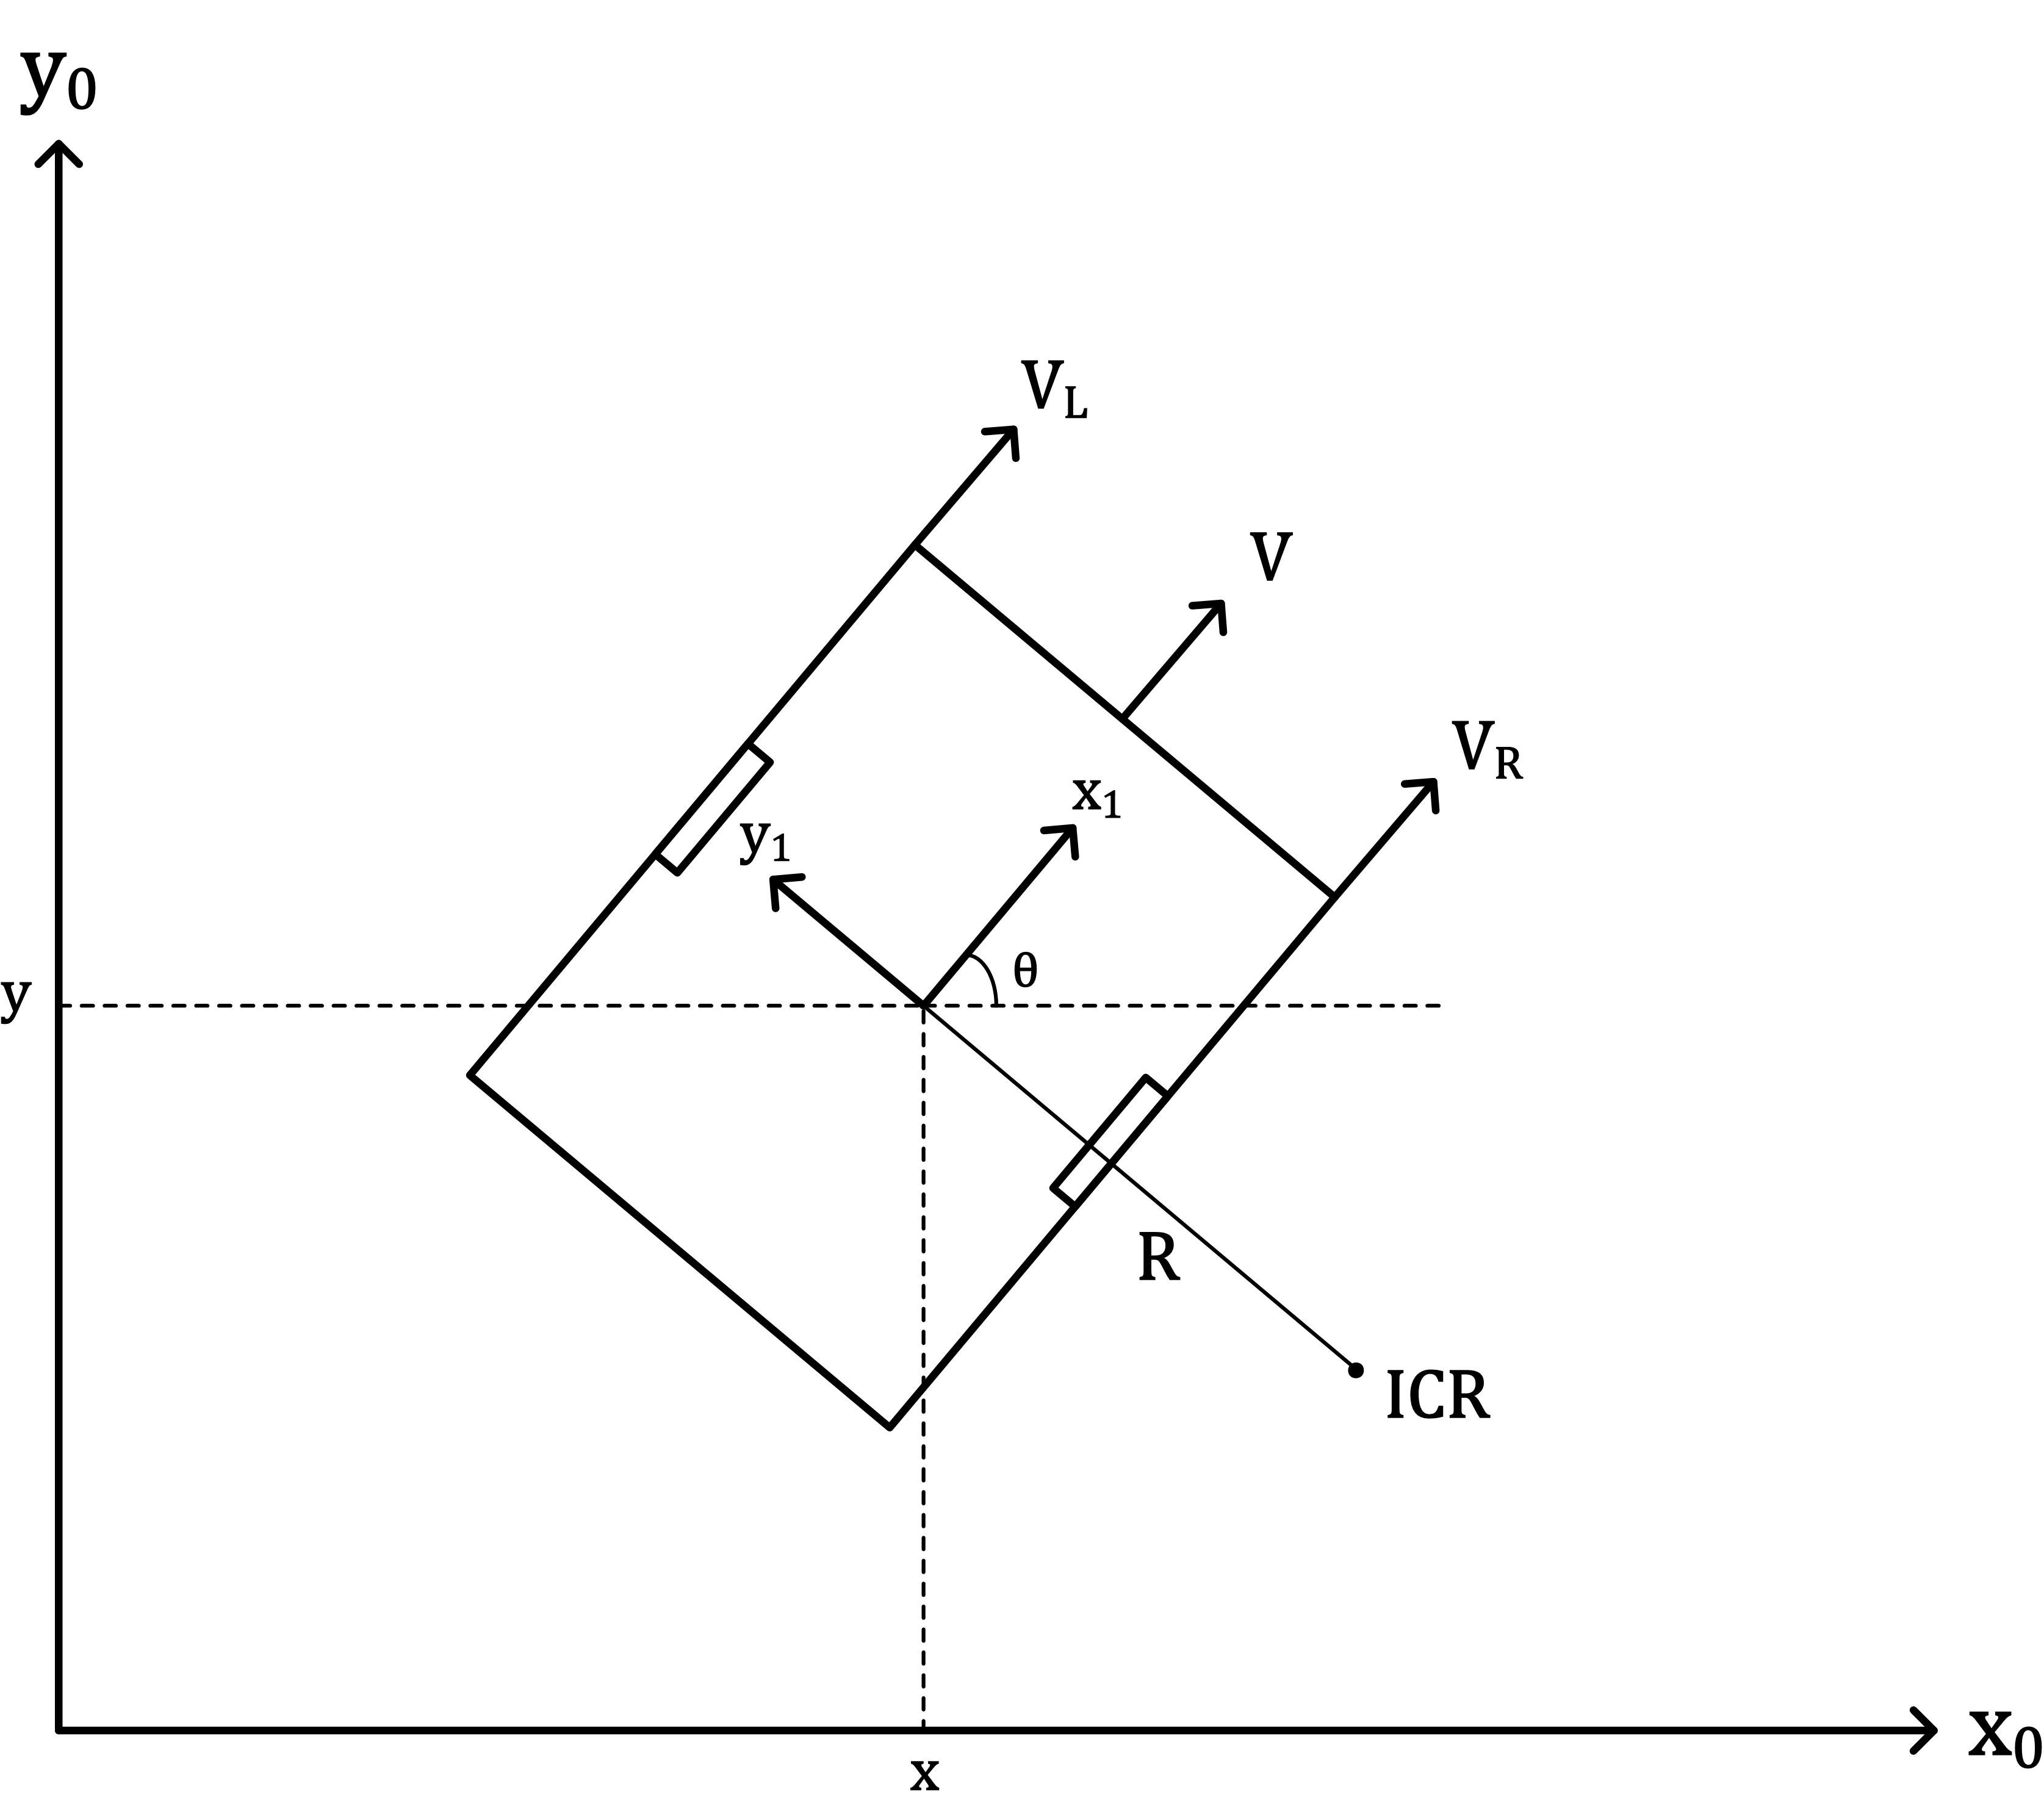
\includegraphics[scale=0.9]{images/kinematics_fig}
	\caption{Frames of a mobile robot in 2D}
	\label{fig:kinematics}
\end{figure}

It is necessary to construct the kinematic model of ITU-AGVs since it will be used in application development. Consider \textit{r} as the radius of the wheels, \textit{R} as the radius of rotation, \textit{L} as the length between the wheels, $\omega$(\textit{t}) and \textit{V}(\textit{t}) as the angular and linear velocities of the robot, \textit{V\textsubscript{L}}(\textit{t}) and $\omega$\textit{\textsubscript{L}}(\textit{t}) as the linear and angular velocities of the left wheel, \textit{V\textsubscript{R}}(\textit{t}) and $\omega$\textit{\textsubscript{L}}(\textit{t}) as the linear and angular velocities of the right wheel, $\theta$ is the angle between x axis of the frames, \textit{x\textsubscript{0}} and \textit{y\textsubscript{0}} as the coordinate axis of the world frame and \textit{x\textsubscript{1}} and \textit{y\textsubscript{1}} as the coordinate axis of the robot frame as in Figure~\ref{fig:kinematics}. 
\par
At any time instant \textit{t}, the linear velocities at left and right wheels can be calculated from the product of their angular velocities and radius;
\par 
\begin{equation}
\textit{V\textsubscript{L}}(\textit{t}) = \omega\textit{\textsubscript{L}}(\textit{t})\cdot\textit{r}
\end{equation}

\begin{equation}
\textit{V\textsubscript{R}}(\textit{t}) = \omega\textit{\textsubscript{R}}(\textit{t})\cdot\textit{r}
\end{equation}

The linear velocities also can be written from the angular velocity of the robot;
\begin{equation}
\textit{V\textsubscript{L}}(\textit{t}) = \omega(\textit{t})\cdot(\textit{R}-\frac{L}{2})
\end{equation}

\begin{equation}
\textit{V\textsubscript{R}}(\textit{t}) = \omega(\textit{t})\cdot(\textit{R}+\frac{L}{2})
\end{equation}

So, combining and solving these equations yields the angular velocity of the robot;
\begin{equation}
\omega(\textit{t}) = \frac{\textit{V\textsubscript{R}}(\textit{t})-\textit{V\textsubscript{L}}(\textit{t})}{L}
\end{equation}

The linear velocity of the robot is simply;
\begin{equation}
\textit{V}(\textit{t}) = \frac{\textit{V\textsubscript{R}}(\textit{t})+\textit{V\textsubscript{L}}(\textit{t})}{2}
\end{equation}

The kinematic model in the world frame can be constructed as;
\begin{equation}
\begin{bmatrix}
\textit{v}_{x\textsubscript{0}}(\textit{t})\\
\textit{v}_{y\textsubscript{0}}(\textit{t})\\
\dot{\theta}(\textit{t})
\end{bmatrix}=
\begin{bmatrix}
cos\theta & 0\\
sin\theta & 0\\
0         & 1
\end{bmatrix}\cdot
\begin{bmatrix}
\textit{V}(\textit{t})\\
\omega(\textit{t})\\
\end{bmatrix}
\end{equation} 

and the kinematic model in the robot frame can be constructed as;
\begin{equation}
\begin{bmatrix}
\textit{v}_{x\textsubscript{1}}(\textit{t})\\
\textit{v}_{y\textsubscript{1}}(\textit{t})\\
\dot{\theta}(\textit{t})
\end{bmatrix}=
\begin{bmatrix}
\frac{r}{2}  & \frac{r}{2}\\
0            & 0\\
-\frac{R}{L} & \frac{R}{L}
\end{bmatrix}\cdot
\begin{bmatrix}
\omega_{L}(\textit{t})\\
\omega_{R}(\textit{t})\\
\end{bmatrix}
\end{equation} 
where $\textit{v}_{x\textsubscript{0}}(\textit{t}),\textit{v}_{y\textsubscript{0}}(\textit{t}),\textit{v}_{x\textsubscript{1}}(\textit{t})$ and $\textit{v}_{y\textsubscript{1}}(\textit{t})$ are the velocities at frame axis $x_{0}, y_{0}, x_{1}$ and $y_{1}$.